\section{SfRequestProvider Class Reference}
\label{classSfRequestProvider}\index{SfRequestProvider@{SfRequestProvider}}
Inheritance diagram for SfRequestProvider::\begin{figure}[H]
\begin{center}
\leavevmode
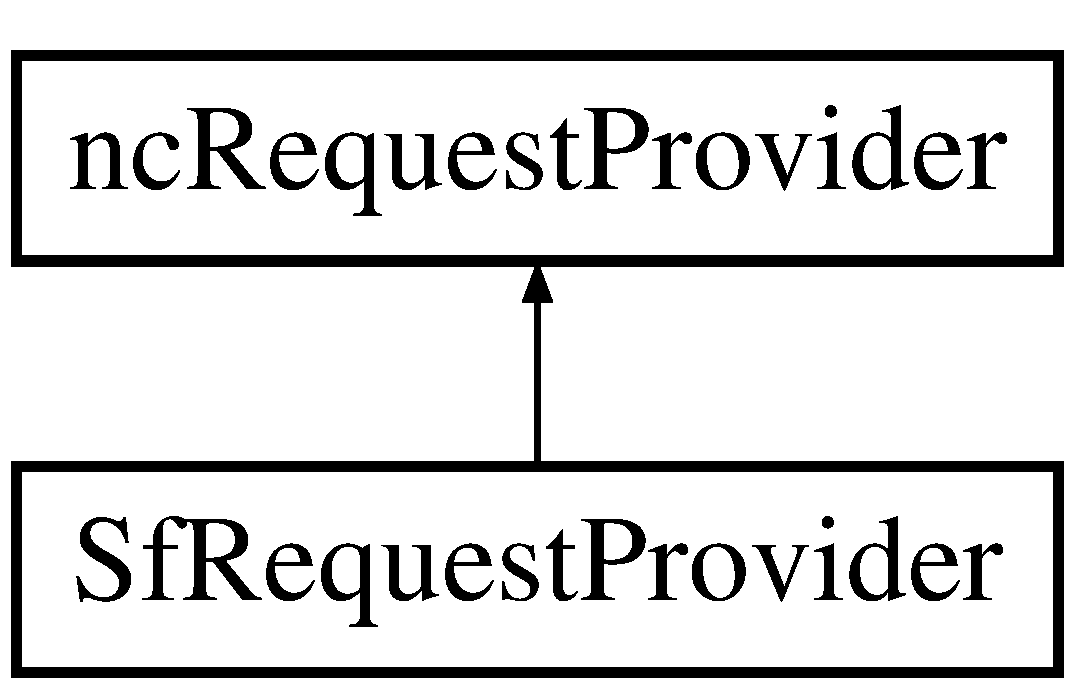
\includegraphics[height=2cm]{classSfRequestProvider}
\end{center}
\end{figure}
\subsection*{Public Member Functions}
\begin{CompactItemize}
\item 
{\bf getRequest} ()
\end{CompactItemize}


\subsection{Member Function Documentation}
\index{SfRequestProvider@{SfRequestProvider}!getRequest@{getRequest}}
\index{getRequest@{getRequest}!SfRequestProvider@{SfRequestProvider}}
\subsubsection{\setlength{\rightskip}{0pt plus 5cm}SfRequestProvider::getRequest ()}\label{classSfRequestProvider_e1694900e5ace5b350415af5157588f3}




The documentation for this class was generated from the following file:\begin{CompactItemize}
\item 
{\bf SfRequestProvider.php}\end{CompactItemize}
